\section{Use Case View}
\label{sec_use_case}

This section lists descriptions of the most significant use cases of the software.

\subsection{Cryptographic Operation on a Message}

Figure \ref{fig:use_case_1} shows a User creating an instance of the SAFEcrypto library that provides a specific scheme and uses a defined parameter set. The User either generates a key-pair or loads a private and/or public key depending upon the intended use. A message is processed by the library in order to provide the cryptographic functionality of the user's application. If necessary, the User encodes the key pair and stores as required. The instance of the SAFEcrypto library is then destroyed.

In another scenario the User maintains a single instance of the SAFEcrypto library, but maintains multiple key pairs associated with different entities. When keys are generated the User obtains the encoded public and private keys for future use or distribution. As the User's application requires cryptographic processing, the relevant key is retrieved and loaded; secure processing can then be performed for communication with a specific entity.

\begin{figure}[H]
\centering
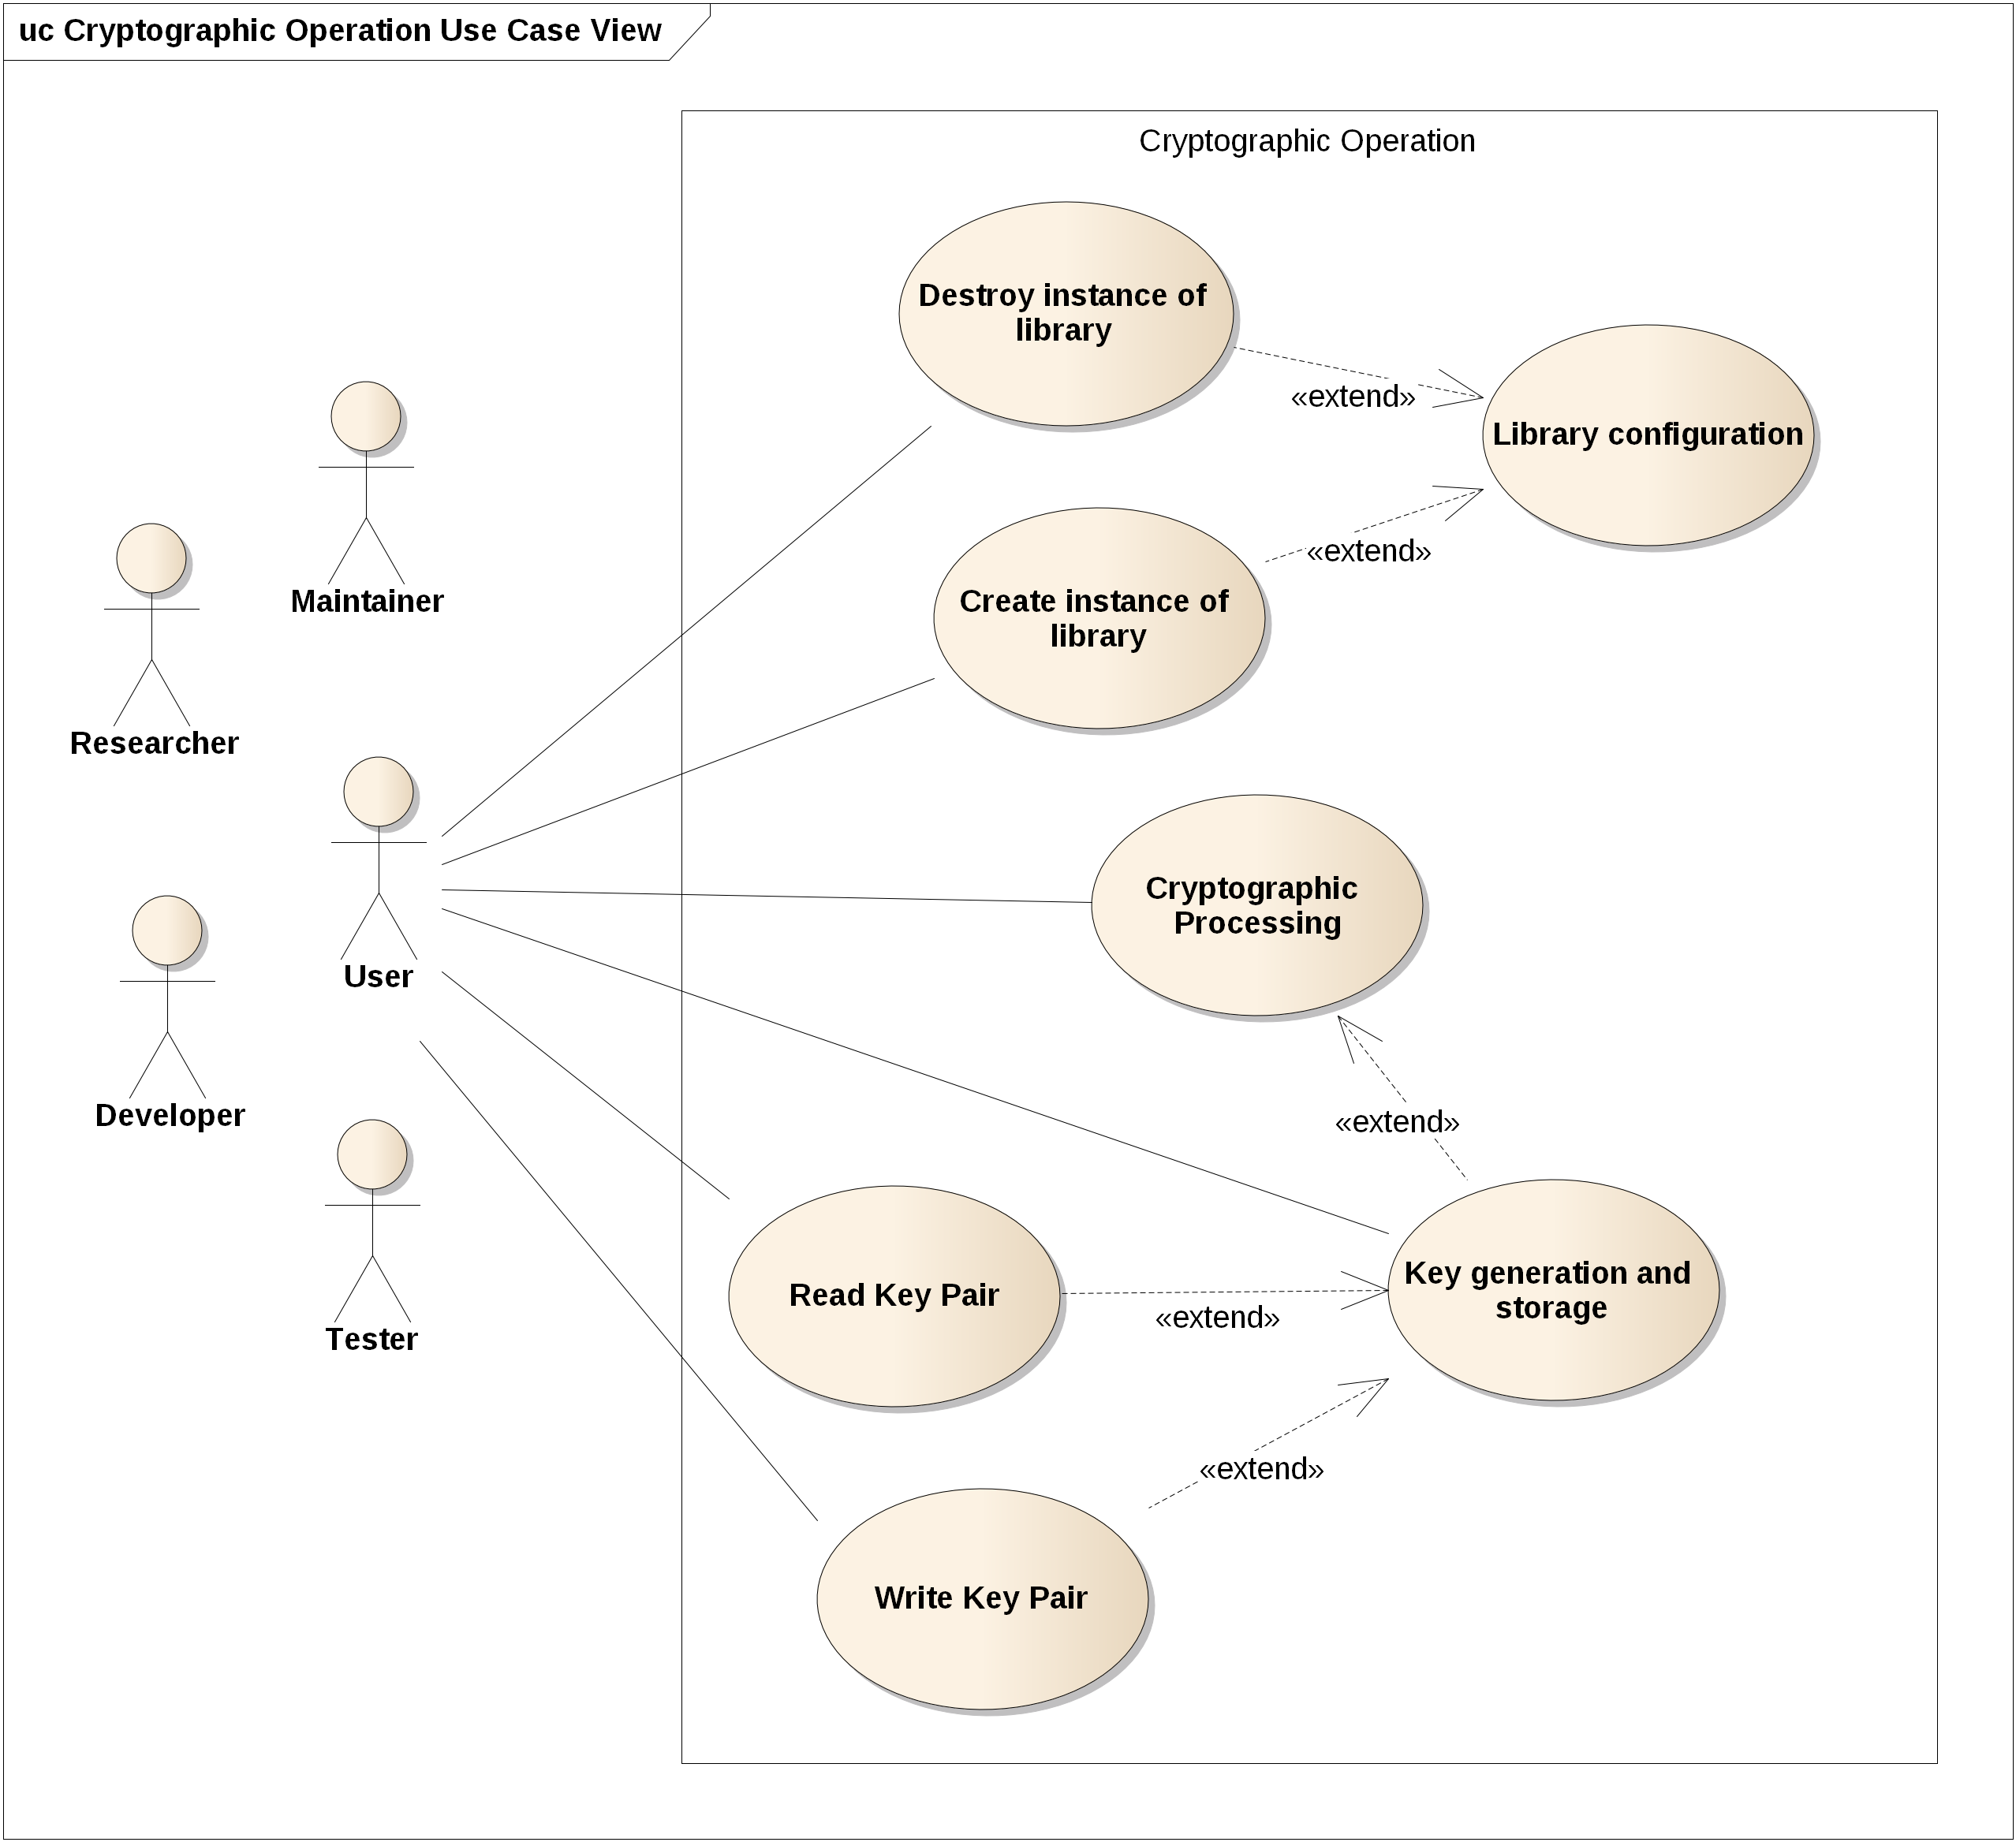
\includegraphics[width=14cm]{cryptographic_operation_use_case_view.png}
\caption{Use case diagram of a message being cryptographically processed}
\label{fig:use_case_1}
\end{figure}


\subsection{Server}

A server application is concerned only with those aspects of cryptographic processing that are necessary to fulfil it's role. A server User will create an instance of the library that does not include any functionality or associated resources for those aspects of a cryptographic application that are not applicable to a server. In many instances a server will have different CPU, memory and transmission bandwidth requirements to that of a client. As such the User will create an instance of the library that is optimally suited to the hardware platform and the target application.

For example, in an IBE network a server User is responsible for generating and maintaining a Master Key from which all User Secret Keys are derived. They are also responsible for the extraction of all User Secret Keys and their subsequent distribution. These are typically memory and compute intensive tasks that are either unsuitable or require design compromises to be made on various hardware platforms.

\begin{figure}[H]
\centering
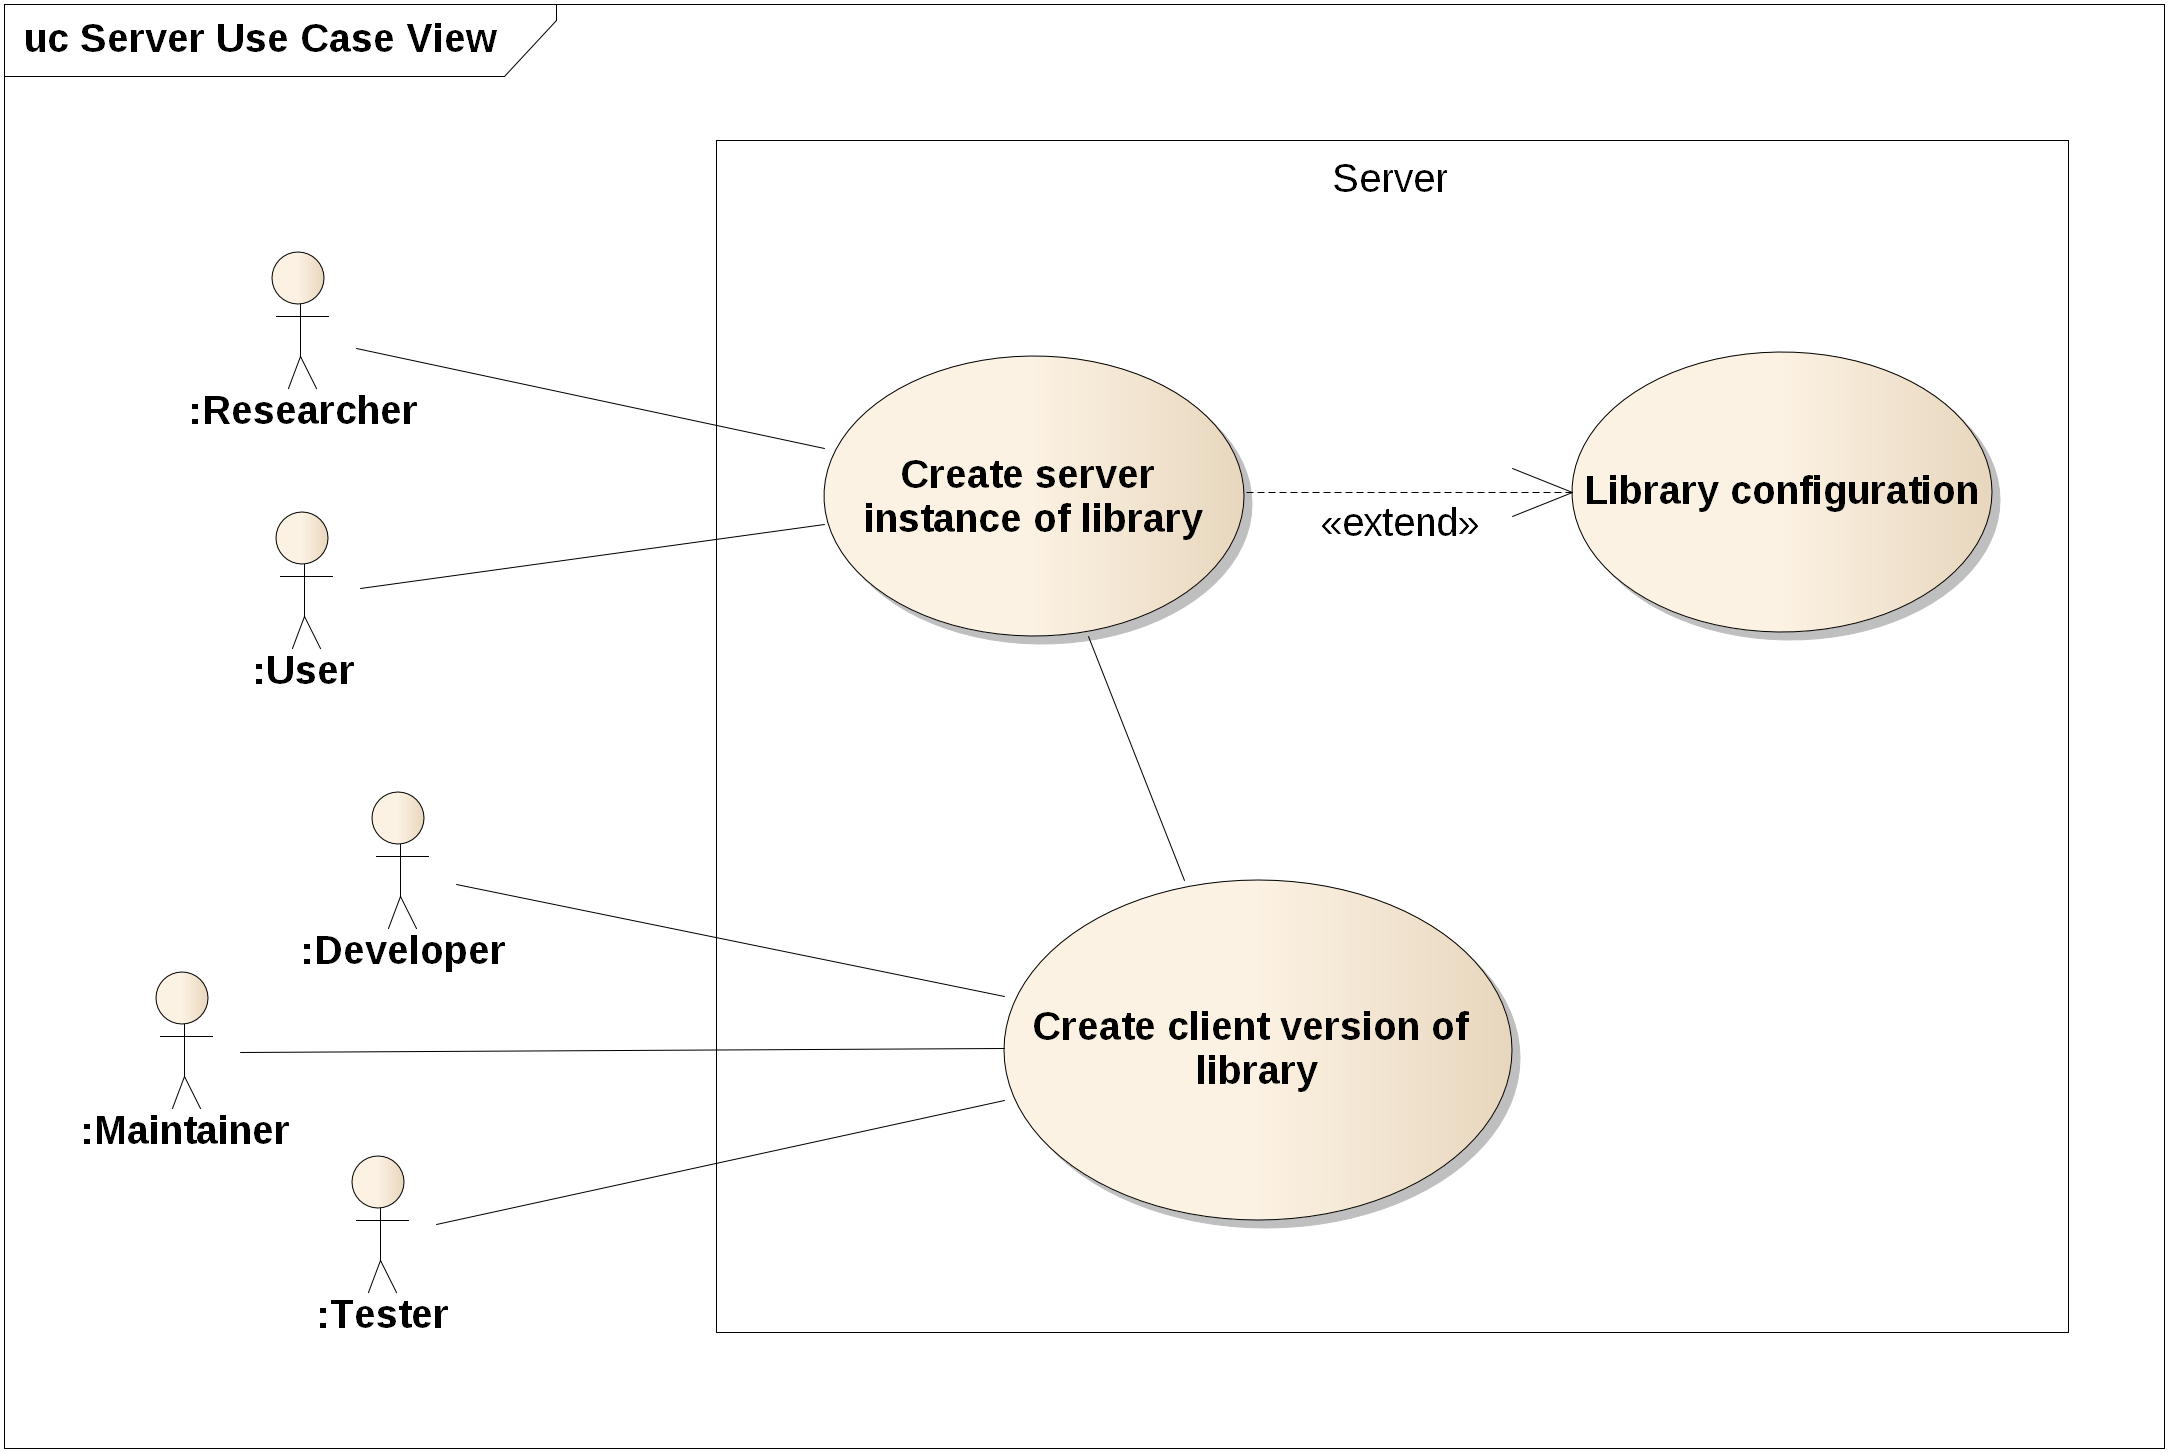
\includegraphics[width=14cm]{server_use_case_view.png}
\caption{Use case diagram of server application}
\label{fig:use_case_2}
\end{figure}


\subsection{Client}

A client application is concerned only with those aspects of cryptographic processing that are neccesary to fulfil it's role. A client User will create an instance of the library that does not include any functionality or associated resources for various aspects of a cryptographic application. In many instances a client application will be deployed on constrained devices where power consumption, memory and processing capabilities are limited. A User created instance of the SAFEcrypto library must be capable of scalability to permit deployment on both constrained devices and high-end servers.

For example, in an Identity-Based Encryption (IBE) application a client User is restricted to performing only Encrypt and Decrypt operations using the User Secret Key provided by a server. A client is not required to perform the computationally intensive tasks of Key Generation or Extraction.

\begin{figure}[H]
\centering
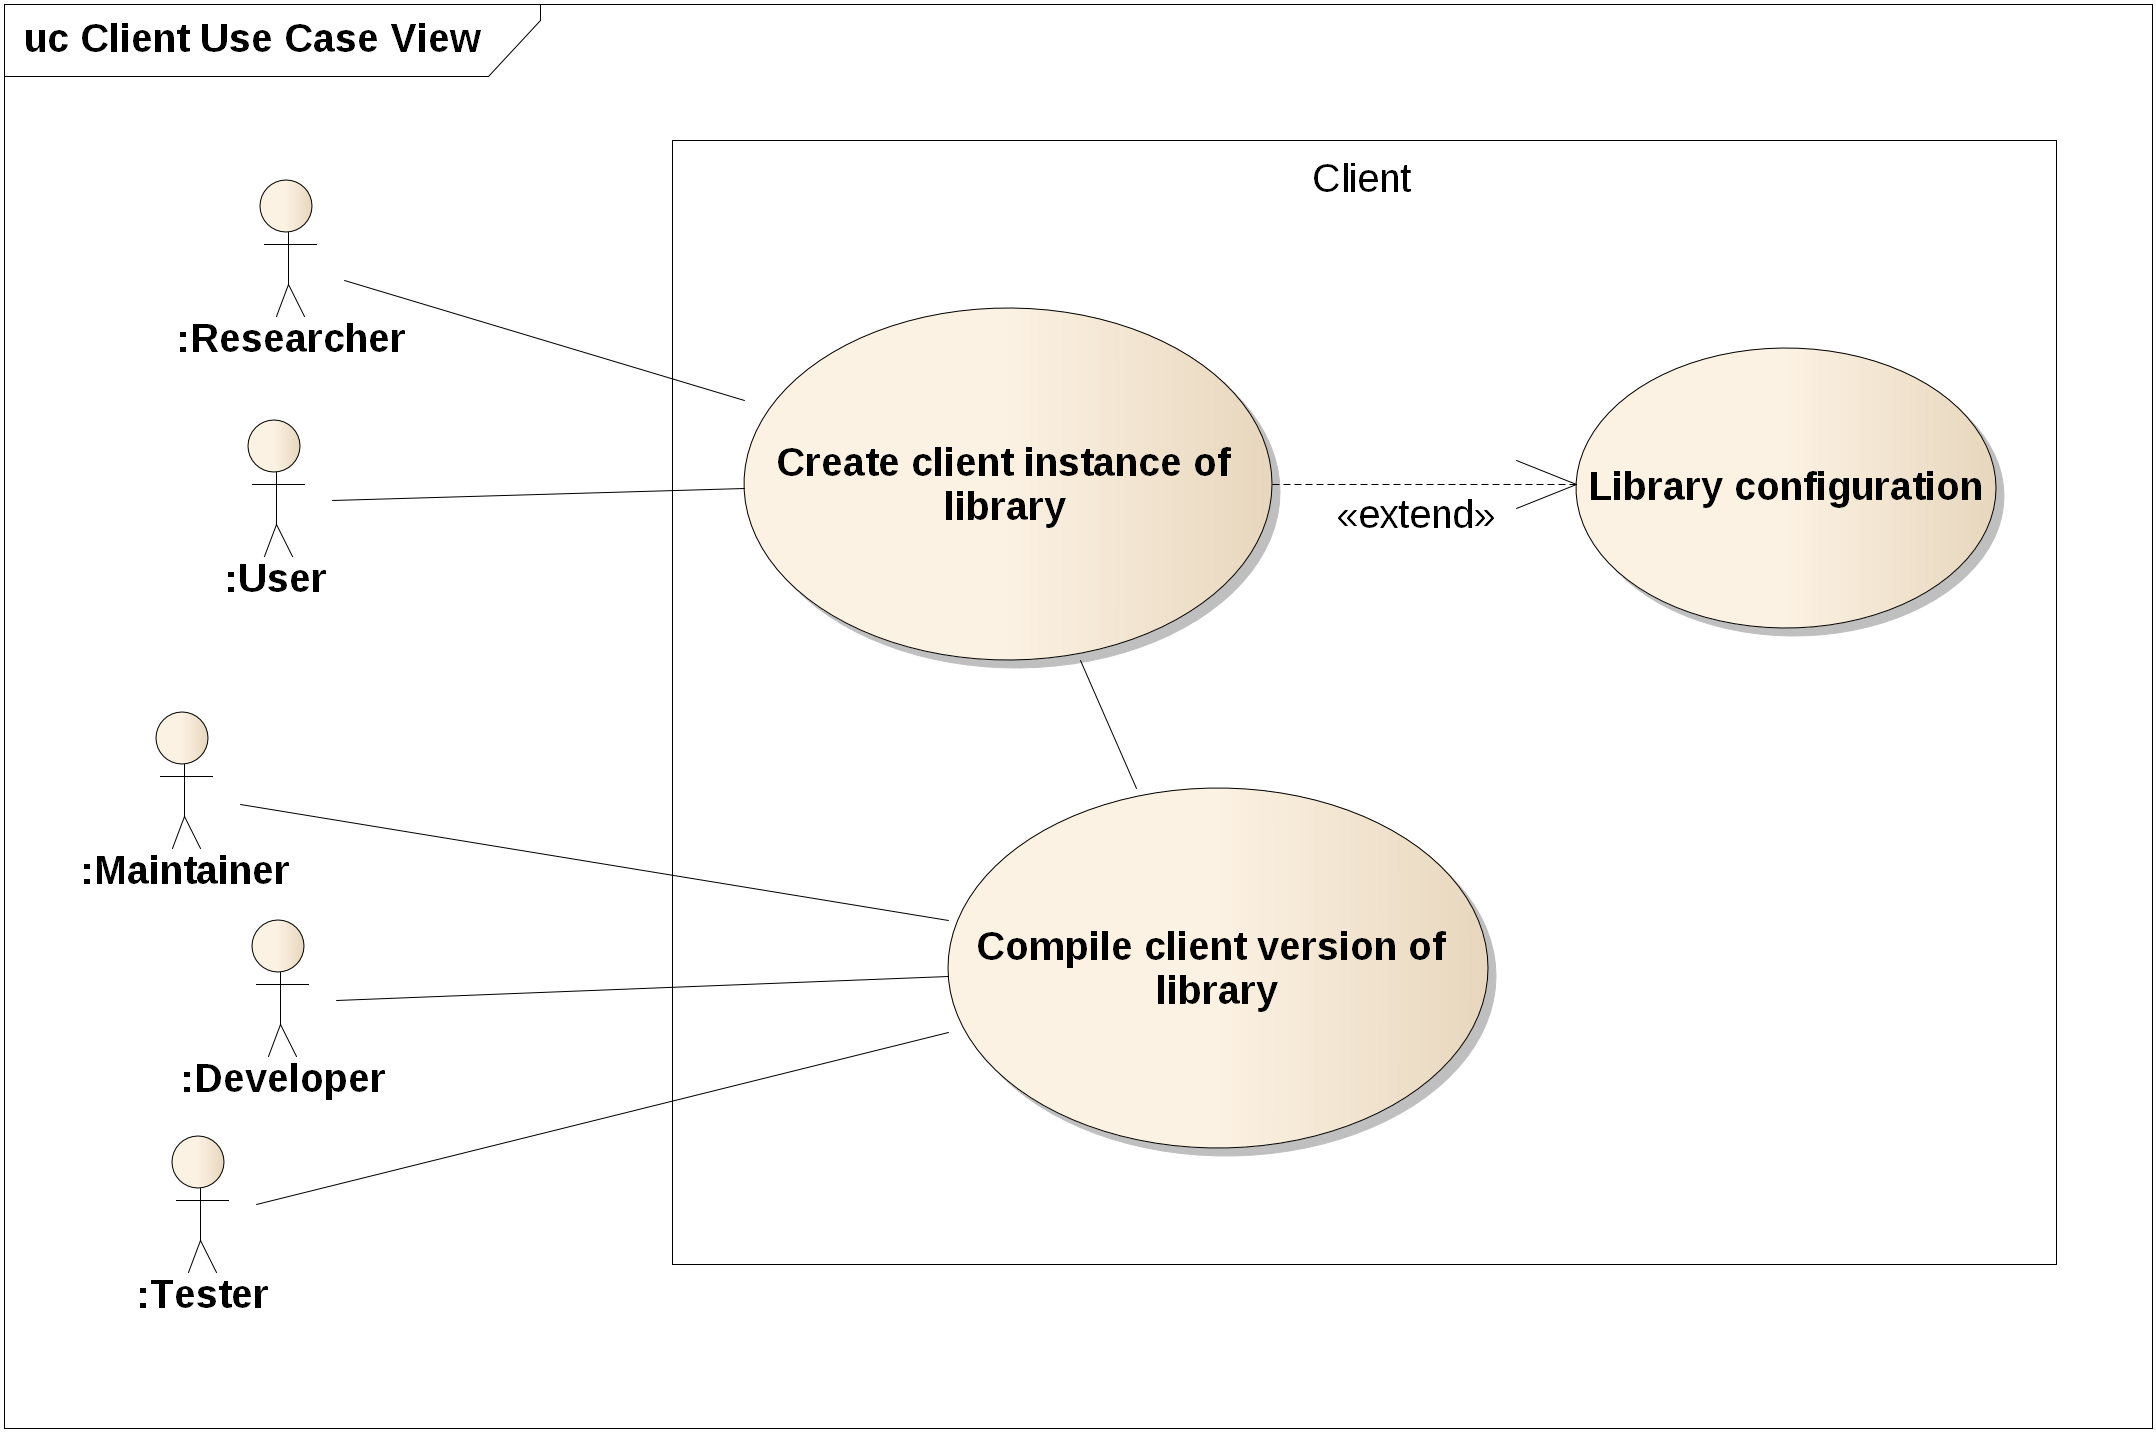
\includegraphics[width=14cm]{client_use_case_view.png}
\caption{Use case diagram of client application}
\label{fig:use_case_3}
\end{figure}


\subsection{Software Integration}

The SAFEcrypto library must be capable of being integrated within a TLS library and an IPSec library for use within the SAFEcrypto project's Use Cases. Integration within both unknown and wide-ranging external software requires that the API offered by the SAFEcrypto library is generic and easily adaptable to different application software which will not necessarily be written in C. This requires that all keys are capable of being loaded and stored such that they can be manipulated by the application software and all data is passed around as generic byte arrays. The library will not perform any complex high level operations such as key management or padding operations of message data, instead leaving such computation to the application level.

In addition, to improve the speed and reliability of the software integration task the SAFEcrypto library must provide extensive test functionality. This will allow the User to both prove the functionality and robustness of the SAFEcrypto library itself, but wwill also provide a description of how the library functions at both an API level and the internal components of the library.

\begin{figure}[H]
\centering
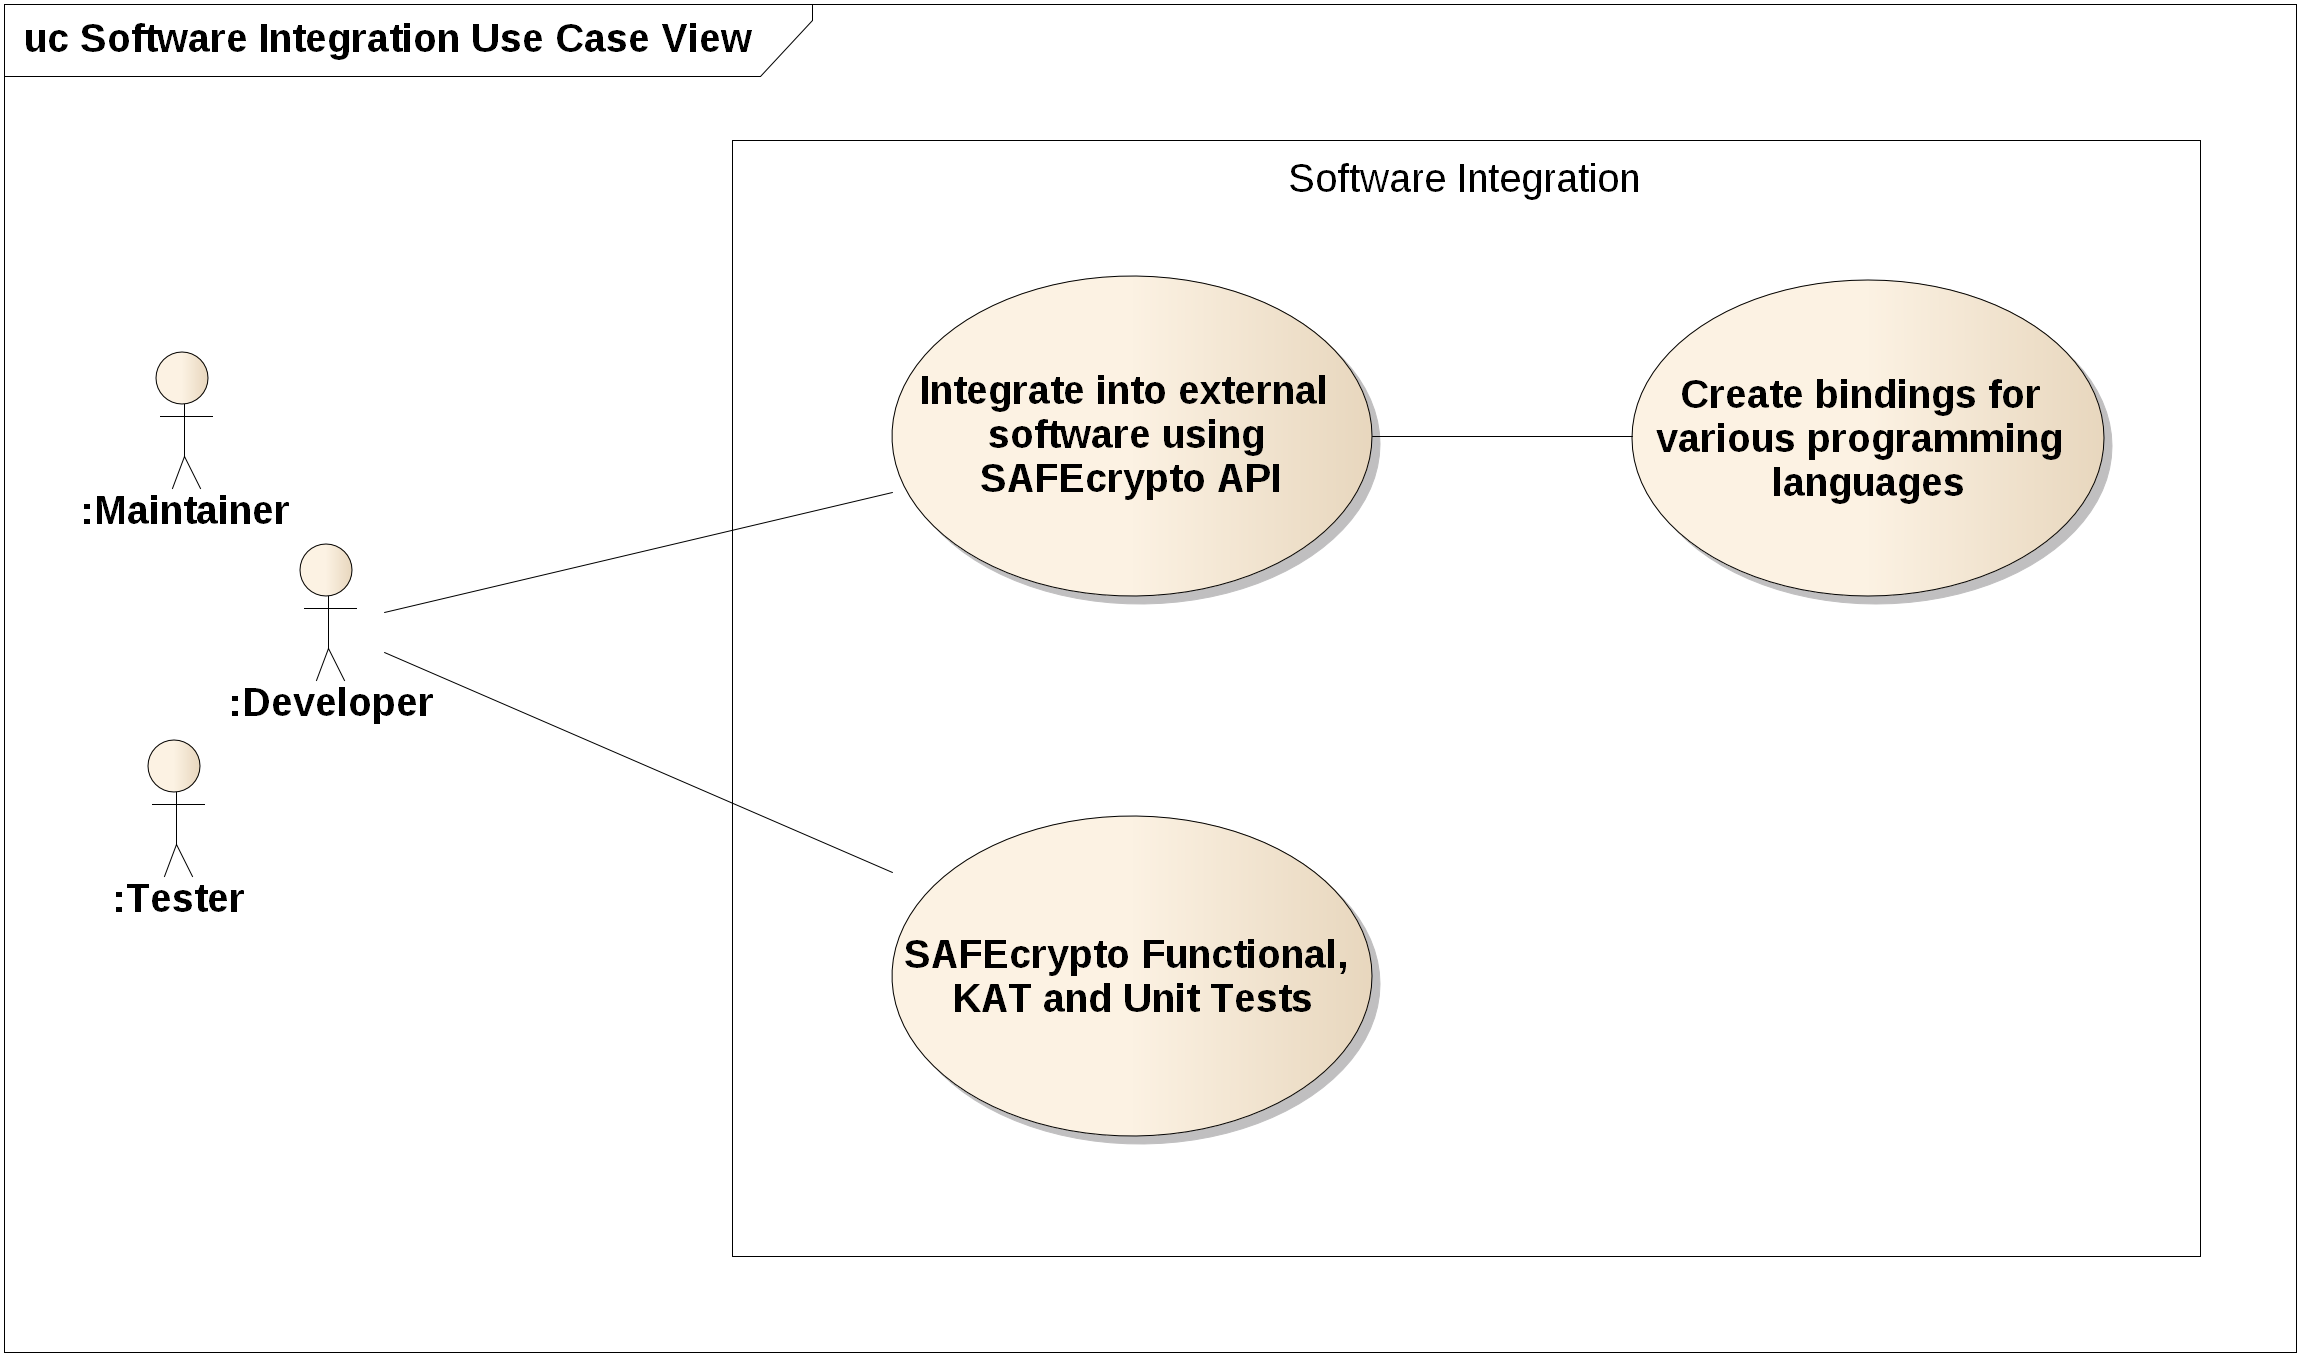
\includegraphics[width=14cm]{sw_integration_use_case_view.png}
\caption{Use case diagram of Software Integration}
\label{fig:use_case_4}
\end{figure}

